\RequirePackage[hyphens]{url}
\documentclass[13pt]{beamer}
\usepackage{beamerthemeshadow}
\usepackage{graphicx}
\usetheme{Szeged}
\usepackage{color}
\usepackage[utf8]{inputenc}
\usepackage{hyperref}
\usepackage{tikz}
\usepackage[flushleft]{threeparttable}
\definecolor{bluebell}{rgb}{0.64,0.64,0.82}
\setbeamercolor{structure}{fg=bluebell}
\usepackage[english, serbian]{babel}
\newcommand\Fontvi{\fontsize{8}{9.2}\selectfont}
\usepackage{array}
\newcolumntype{C}[1]{>{\centering\arraybackslash}m{#1}}

\def\d{{\fontencoding{T1}\selectfont\dj}}
\def\D{{\fontencoding{T1}\selectfont\DJ}}


\title{Medijska pismenost}
\author{Ljiljana Mihajlović, \and Danica Šimšić, \and Ana Stevanović, \and Tijana Zečević}
\institute{Matematički fakultet \\Univerzitet u Beogradu}
\date{
	\footnotesize{Beograd, 2022.}	
}

\begin{document}
\begin{frame}
	\thispagestyle{empty}
	\titlepage
\end{frame}

\addtocounter{framenumber}{-1}

\begin{frame}
	\begin{itemize}
		\item Zasnovano na:\\
        \begin{itemize}
		\item Grupa autora (po azbučnom redu): Vlajković Bojić Violeta, Miladinović Nenad, Milijić Subić Dejana, Milošević Ivana. Priručnik za nastavnike \emph{ Naši učenici u svetu kritičkog mišljenja i medijske pismenosti}.
		(\url{https://zuov.gov.rs/prirucnik-za-nastavnike-nasi-ucenici-u-svetu-kritickog-misljenja-i-medijske-pismenosti/})


      \item  Nedim Sejdinović i Tatjana Ljubić, \emph{Osnove medijske pismenosti– priručnik za učenike}, 2014.
         (\url{http://www.medijskapismenost.net/dokument/Osnove-medijske-pismenosti---prirucnik-za-ucenike/})\\
           \end{itemize} 

	\end{itemize}
\end{frame}

\begin{frame}
	\frametitle{Pregled} % Table of contents slide, comment this block out to remove it
	\tableofcontents[hidesubsections] 
\end{frame}

\section{Tradicionalni i društveni mediji}

\begin{frame}[fragile]\frametitle{Tradicionalni i društveni mediji}
	\begin{itemize}	
		\item \textbf{Mediji} se definišu kao različiti kanali ili načini pomoću kojih se šire vesti, zabava, marketinške poruke ili druge informacije.

		\item \textbf{Tradicionalni mediji:}\begin{itemize}
            \item svi vidovi štampanih medija
	    \item televizija
		\item radio
		\item pošta i poruke na javnim mestima
            \end{itemize}
		\item \textbf{Društveni mediji} \begin{itemize}
            \item Veb lokacije i aplikacije
            \end{itemize}
	\end{itemize}

 
 \begin{tikzpicture}[remember picture, overlay]
\node[below = 3.2cm, left=1.7cm] at (current page.0)  
{
    
\includegraphics[width=0.20\textwidth]{newspaper.jpg}
     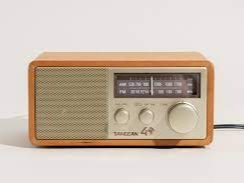
\includegraphics[width=0.20\textwidth]{radio.jpg}
      
\includegraphics[width=0.20\textwidth]{tv.jpg}
       
\includegraphics[width=0.20\textwidth]{ikonice.jpg}
};
\end{tikzpicture}
\end{frame}

\section{Spinovanje i manipulacija}

\begin{frame}[fragile]\frametitle{Spinovanje: metode medijske manipulacije}
	\begin{itemize}	
		\item Preusmeravanje pažnje
		\item Selektivno predstavljanje činjenica
		\item Stvaranje problema
  	\item Upotreba dečijeg jezika
		\item Stvaranje osećaja krivice
		\item Buđenje emocija
	\end{itemize}
 \begin{tikzpicture}[remember picture, overlay]
\node[below=2.5cm, left=1cm] at (current page.east) 
{
    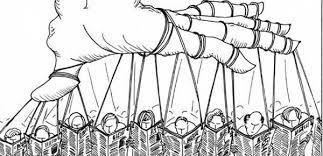
\includegraphics[width=0.5\textwidth]{spinovanje.jpg}
};
\end{tikzpicture}
\end{frame}


\section{Dezinformacije}
\begin{frame}[fragile]\frametitle{Dezinformacije: vidovi i načini prepoznavanja}
	\begin{itemize}	
		\item podmetnuti sadržaj
		\item obmanjujući sadržaj
		\item fabrikovani sadržaj
  		\item manipulisani sadržaj
	\end{itemize}
 
\begin{tikzpicture}[remember picture, overlay]
\node[above=0.7cm, left=1cm] at (current page.east) 
{
    
\includegraphics[width=0.5\textwidth]{fakewebsite.jpg}
};
\end{tikzpicture}

\begin{tikzpicture}[remember picture, overlay]
\node[below = 2.65cm, left=1cm] at (current page.0) 
{
    
\includegraphics[width=0.5\textwidth]{takecarebeforeyoushare.jpg}
};
\end{tikzpicture}

\end{frame}

\section{Medijska pismenost u doba informacija}

\begin{frame}[fragile]\frametitle{Medijska pismenost u doba informacija}
	\begin{itemize}	
		\item Definicija pismenosti kroz godine
		\item Medijska pismenost - sposobnost razumevanja,\\ korišćenja i adekvatne interpretacije\\ medijskih poruka
		\item Vrste pismenosti u digitalnom dobu
        \item Da li mi biramo informacije \\ili one nas?
	\end{itemize}

 \begin{tikzpicture}[remember picture, overlay]
\node[below = 1.8cm, left=0.01cm] at (current page.0)  
{
    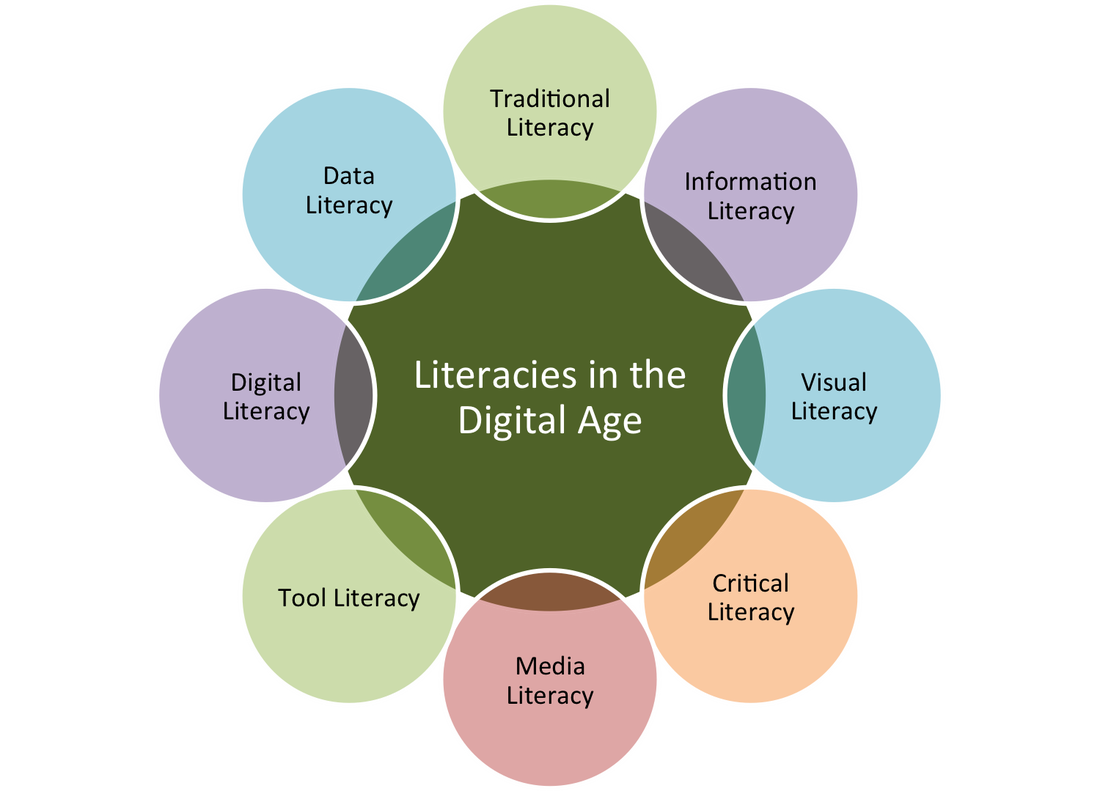
\includegraphics[width=0.58\textwidth]{literacies.png}
};
\end{tikzpicture}
\end{frame}

\begin{frame}[fragile]\frametitle{Tabela za analizu medijskog sadržaja}
\Fontvi
\begin{table}[h!]
\begin{center}
\begin{tabular}{|m{1.5cm}|m{4cm}|m{4cm} |} \hline
Ključne reči& Ključna pitanja& Suštinski koncepti\\ \hline
Autorstvo&Ko je napisao poruku?&Sve medijske poruke su "konstruisane".\\ \hline
Format &Koje kreativne tehnike se koriste kako bi se privukla moja pažnja?&Medijske poruke su konstruisane upotrebom kreativnog jezika sa sopstevnim pravilima.\\ \hline
Publika &Kako različiti ljudi mogu ovu poruku razumeti drugačije od mene?&Različiti ljudi doživljavaju istu medijsku poruku na različit način.\\ \hline
Sadržaj &Koje vrednosti, životni stilovi i gledišta se prikazuju ili izostavljaju iz ove poruke?&Svaki medij ima ugrađene vrednosti i tačke gledišta.\\ \hline
Svrha &Zbog čega se ova poruka šalje?&Većina medijskih poruka je kreirana sa ciljem da ostvari profit i/ili moć.\\ \hline
\end{tabular}
\caption{Koraci za analizu medijskog sadržaja}
\label{tab:tabela2}
\end{center}
\end{table}
\end{frame}

\section{Zaključak}

\begin{frame}[fragile]\frametitle{Zaključak}
		\begin{itemize}	
			\item Medijska pismenost je važna zato što nas uči da tumačimo različite vrste medija, razumemo informacije i njihov izvor postavljajući prava pitanja, razlikujemo činjenice od mišljenja 
			\item  Pomaže nam da razlikujemo stvarnost od sveta koji su kreirali mediji.
			\item Važno je pomenuti da mediji bitno utiču na uspostavljanje društvenog sistema vrednosti. 
		\item Medijska pismenost nas uči da razlučimo kojim medijima treba verovati, kao i da uvek treba proveriti određenu informaciju, pre nego što je objavimo ili podelimo
        \end{itemize}
\end{frame}

\end{document}
